\section{Introduction}
In this paper, we study a variant of the classic Art Gallery problem, where the goal is not to minimize the number of guards required to cover a region, but instead to maximize the portion of the polygon's boundary that is guarded by a budgeted number of guards. Specifically, given a simple polygon $P$ and $k\in\mathbb{N}$, we want to find the $k$ vertex guards which maximize the length of the boundary of $P$ that is watched. We define the set of vertices of $P$ as $V_P$, and $L(S)$ as the length of the boundary seen by the set of vertex guards/vertices $S$. Note that $L(S)$ is necessarily at most the perimeter of $P$. 

\optproblemdef{\MLVG{}}{A simple polygon $P$ and a positive integer $k\in\mathbb{N}$.}{Find a set of vertices $S\subseteq V_P$ of size at most $k$ such that $L(S)$ is maximized.}

We also study a weighted version of the problem, where the polygon $P$ is composed of (possibly collinear) boundary segments, each assigned a non-negative integer weight. An example of such a polygon is shown in~\Cref{fig:weighted-polygon}. This models a more realistic art gallery, where some sections of the wall (e.g., those holding more valuable paintings) are more important to guard than others, especially when the constrained number of guards may prevent us from guarding the entire gallery. In this variant, the goal is to maximize the total weight of boundary segments that are \emph{fully} visible to the vertex guards. We define $W(S)$ as the weighted analog of $L(S)$: the sum of the weights of all boundary segments that are completely seen by the guard set $S$.

\begin{figure}
    \centering
    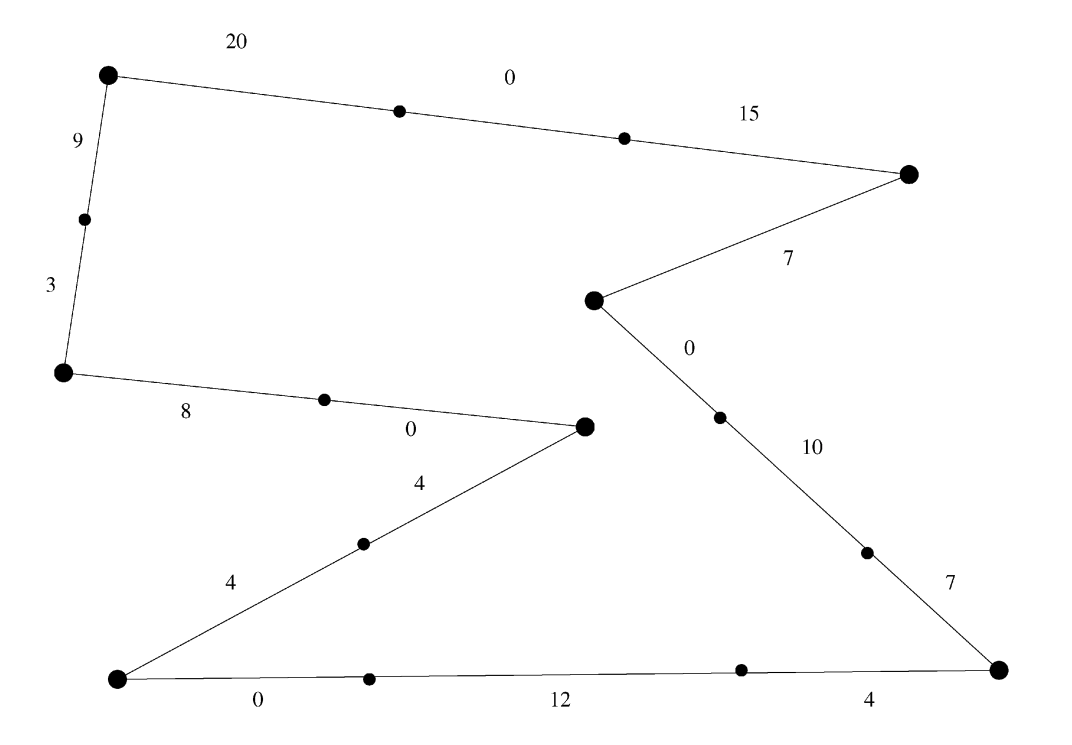
\includegraphics[width=10cm]{figures/weighted-polygon.png}
    \caption{A polygon composed of weighted line segments, the input for \MVVG{}.}
    \label{fig:weighted-polygon}
\end{figure}

\optproblemdef{\MVVG{}}{A weighted polygon $P$ and a positive integer $k\in\mathbb{N}$.}{Find a set of vertices $S\subseteq V_P$ of size at most $k$ such that $W(S)$ is maximized.}

Finally, we consider a budgeted variant of \MVVG{}, where each vertex has an associated placement cost. This is in contrast to \MVVG{}, where the constraint was the number of guards, not the total guard cost. Depending on the setting, it may be more difficult or expensive to position a guard at certain locations of the art gallery, and this problem formulation captures that added difficulty. Now, instead of selecting up to $k$ guards, we are given a total budget $B$, and each vertex $v$ has a cost $c(v)\leq B$. The goal is to choose a set of guards whose total cost does not exceed $B$, while maximizing the total weight of boundary segments they fully guard.

\optproblemdef{\BMVVG{}}{A weighted polygon $P$ and a positive integer $B\in\mathbb{N}$.}{Find a set of vertices $S\subseteq V_P$ with $\sum_{s\in S}c(s)\leq B$ such that $W(S)$ is maximized.}

\subsection{Related Works}
The Art Gallery problem, originally posed by Victor Klee to Václav Chvátal in 1973, is a foundational problem in computational geometry with numerous variations. In its original form, the problem asks for the minimum number of guards required to fully guard the interior of a simple polygon $P$ with $n$ vertices. A comprehensive overview of early results is provided in \cite{orourke-artgallery}, which includes both foundational combinatorial results and a survey of the state of the field (as of 1987).\\\\
Subsequent research has explored the problem through the lens of approximation algorithms. It is now known that the Art Gallery problem is $O(\log n)$-approximable and \cclass{APX}-complete, meaning that no polynomial-time approximation scheme (PTAS) exists unless \cclass{P} = \cclass{NP}. Recent work, such as \cite{das-robustly}, introduces novel approximation strategies and includes a comprehensive literature review of prior approximation results for the Art Gallery problem. Additional inapproximability results are presented in \cite{abdelkader}, which considers restricted visibility models where guards have a limited field of view.\\\\
This paper focuses on a boundary-maximization variant of the Art Gallery problem, where the objective is to maximize the length of the polygon boundary that is fully guarded, rather than minimizing the number of guards. This formulation was introduced by Fragoudakis et al.\ in a series of papers \cite{fragoudakis-interior, fragoudakis-boundary, fragoudakis-paintings}, where they introduce and study both the \MLVG{} and \MVVG{} problems. In \cite{fragoudakis-boundary}, they show that both problems are \cclass{APX}-complete. In \cite{fragoudakis-interior}, they present a $(1-1/e)$-approximation algorithm for maximizing the vertex-guarded interior area of a polygon, based on partitioning the polygon into what they call the Finest Visibility Segmentation. Their algorithm runs in $O(k^2n^2)$ time.\\\\
Our work also draws heavily on the relationship between the Set Cover problem and various Art Gallery formulations. Specifically, we use techniques from the Max $k$-Coverage problem to inform our approach to \MLVG{}. \cite{hochbaum-maxkcover} analyzes the Max $k$-Coverage problem and provides tight approximation bounds. These connections also position our work within the broader study of optimizing monotone submodular functions under cardinality constraints, where $(1-1/e)$-approximation factors are both the best known and provably optimal (assuming $\cclass{P}\neq\cclass{NP}$) for cardinality-constrained maximization \cite{cornuejols,feige}.
In addition to cardinality constraints, we also study a budgeted version of \MVVG{}, where each vertex has an associated cost. This leads us to consider the budgeted Max $k$-Coverage, which was introduced in \cite{khuller} and also admits a $(1-1/e)$-approximation algorithm under a total cost constraint.

\subsection{Our Contributions}
For both \MLVG{} and \MVVG{}, we improve upon the $(1-1/e)$-approximation algorithm with $O(k^2n^2)$ running time from \cite{fragoudakis-interior,fragoudakis-boundary,fragoudakis-paintings} by proving that the objective function in each case is monotone and submodular. This structural property allows us to apply the standard greedy algorithm for submodular maximization, yielding a $(1-1/e)$-approximation that runs in $O(kn^2)$ time. We further show that this approximation ratio is optimal unless \cclass{P} = \cclass{NP}, aligning with their prior result that both problems are \cclass{APX}-complete.\\\\
We also introduce a budgeted variant of \MVVG{}, called \BMVVG{}, where guards have associated costs and the goal is to maximize the total weight guarded under a fixed budget, rather than a cardinality constraint. We demonstrate that three natural greedy strategies fail to form an approximation:
\begin{enumerate}
    \item Greedily selecting the vertex which provides the highest marginal gain in total weight guarded.
    \item Greedily selecting the cheapest vertex.
    \item Greedily selecting the vertex which provides the highest ratio of marginal gain in total weight guarded to vertex cost.
\end{enumerate}
Using these counterexamples as motivation, we propose an algorithm inspired by \cite{khuller} that may achieve a $\frac{1}{2}(1-1/e)$-approximation for \BMVVG{}.

